In this chapter, detailed description of NF chaining mechanism in kernel space is given. 

The design of the Kernel-based NFCI is shown in Figure \ref{fig: design}. All the arrived packets are first checked by the registered rules that determines which flow should be processed by which NF chain. If the packet matches a rule the corresponding NF chaining starts. The NFs in the chain are executed in registered order. Each NF processes packets by directly accessing with pointer. 
 
 \begin{figure*}
	\centering
	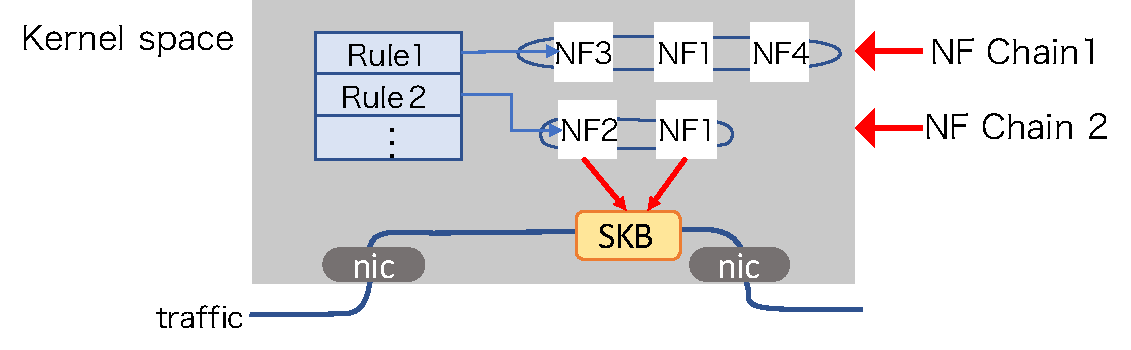
\includegraphics[width=120mm]{pics/design.pdf}
	\caption{Design of the Kernel-based NFCI.}
	\label{fig: design}
\end{figure*}

Kernel-based NFCI has three main components. One is the identification of flow. The second is chaining of NFs, the system that enables packets to be processed by NFs in order. And the last is the NFs themselves. Any kind of NF consists of one kernel module or more. The NF chaining mechanism takes place in the PRE\_ROUTING hook which locates between hardware and routing subsystem in the network stack, which is called here chaining point. 

\subsection{Network Function}
Any installed kernel modules exist in the same memory region as kernel so the functions in the modules can be seen from other modules and from kernel. This is why it is possible to call functions in kernel modules from network stack. Normally a NF consists of several kernel modules. And in this case, the very first function among kernel modules should be registered somewhere in the kernel and the subsequent functions in other kernel modules will be called in order. 

\subsection{Identification of flow}
In the kernel-based NFV host, sets of NF chain can be registered. When a network node participates in NF chaining, it is likely that many flows comes in and out. Not all the flows are to be processed by a single NF chain but only specific flows should pass its designated NF chains. So a mechanism is needed to specify which kind of flow should be treated by a chain of NFs in the host. For example in OPNFV, OVS is used to direct flows to the right NFs which are in VMs. OVS employs OpenFlow which can set a very detailed rules using VLAN tag, incoming / outgoing port, etc. Kernel-based NFV distinguishes flows in granularity of five tuples. Five tuples represent source / destination IP address, source / destination port number and the transport protocol. 

The identification of flow in 5-tuple is implemented using Filter table. As explained in Sec. 4.1.2, Filter table carries out filtering by setting rule and verdict of NF\_DROP or NF\_ACCEPT. Instead of setting verdict in the target, pointer to the list head of chained NFs is registered. 

\subsection{Chaining of Network Functions}
This mechanism uses Doubly Linked List (DLL) to implement NF chaining. DLL is a list that contains links to next and previous nodes. Unlike singly linked lists traversal is only one way, DLL allows traversal in both ways. 
Figure \ref{fig: dll} shows the framework of NF chain realized with DLL. DDL is chosen since adding and removing node can be done easily. A NF is represented by a node of gray box. A node is a {\tt nf\_target} struct which has the following members: 
\begin{itemize}
	\item {\tt list\_head} struct : {\tt list\_head} struct has two pointers, next and prev, which respectively points to the previous node and next node. 
	\item pointer to function : This points to the function in the kernel module. The function will execute the process of NF.
	\item priority : This is a integer value that is used to put the {\tt nf\_target} struct in the right position in the DLL. The smaller the value is, the higher the priority is.
\end{itemize}

\begin{figure*}
	\centering
	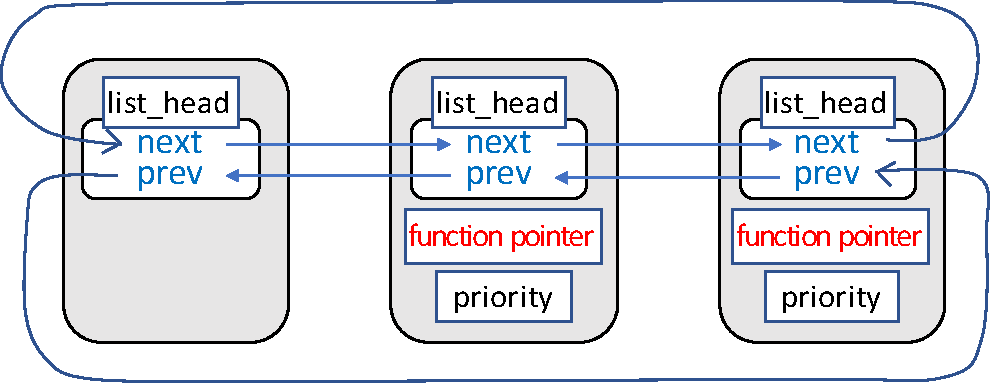
\includegraphics[width=90mm]{pics/dll.pdf}
	\caption{Doubly Linked List with nodes of {\tt nf\_target} struct.}
	\label{fig: dll}
\end{figure*}

\begin{figure*}
	\centering
	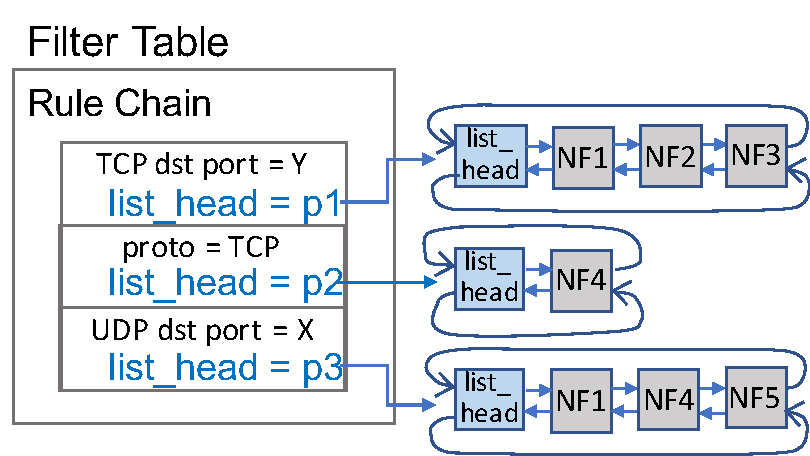
\includegraphics[width=90mm]{pics/list_head.pdf}
	\caption{Structure of rules and the corresponding NF chain in Filter Table.}
	\label{fig: listhead}
\end{figure*}

 When inserting a NF in a chain, the priority and the function to be registered must be given. According to this information and network namespace, a {\tt nf\_target} struct is created and inserted in the corresponding DLL. The struct is inserted before the node that has higher priority. 
 
 Figure \ref{fig: listhead} shows the example of Filter table and how the DLL that represents NF chain is linked. The mechanism that is responsible for NF chaining is called NFC system from here. When a packet arrives at the chaining point, it first traverses the Filter table to be passed to the right NF chaining. If a rule matches, the corresponding chaining starts: The NFC system takes the list head of the registered NF chain from the target component. Now from the next node in the DLL, which is the first NF, starts the process. The pointer to the SKB (Socket Buffer) is passed to the registered function in the node which will starts the entire the NF process. When the process is finished, the control comes back to the NFC system. At this point the function in the node returns verdict as well. There are only two types of them, DROP or ACCEPT. If it returns DROP, the NFC system stops the chaining and the SKB will be freed. Otherwise the system pass the SKB pointer to the function in the next node to process the next NF. The same procedure will continue until the last NF in the chain is executed. When the last NF returns ACCEPT, the NFC system ends NF chaining for the SKB and it will move to the next stage of network stack. 

As an example, when a UDP packet with destination port X arrives at the Filter table configured like Fig. \ref{fig: listhead}, the first and second NF chains are skipped. And the packet matches the last rule so the NF chaining of NF1, NF4 and NF5 starts. If all functions of NFs return ACCPET, this SKB that is probably modified by three NFs continues its journey in the network stack. 
